%%%%%%%%%%%%%%%%%%%%%%%%%%%%%%%%%%%%%%%%%%%%%%%%%%%%%%%%%%%%%%%%%%%%%%%%
%                                                                      %
%     File: Thesis_Introduction.tex                                    %
%     Tex Master: Thesis.tex                                           %
%                                                                      %
%     Author: Andre C. Marta                                           %
%     Last modified :  2 Jul 2015                                      %
%                                                                      %
%%%%%%%%%%%%%%%%%%%%%%%%%%%%%%%%%%%%%%%%%%%%%%%%%%%%%%%%%%%%%%%%%%%%%%%%

\chapter{Introduction}
\label{chapter:introduction}

With the advent of Big Data, a massive amount of information is constantly being collected and analyzed to extract value out of it. The way to obtain the value is through the use of machine learning (ML) algorithms, capable of analyzing huge data sets and uncover relations and extract meaning out of the raw information. These algorithms are being run in all kinds of devices, from supercomputers to our smartphones and a tonic exists across all kinds of modern devices, they are Heterogeneous Computing Systems composed of traditional Central Processing Units (CPUs) and Graphical Processing Units (GPUs). The use of GPUs, with their highly parallel architecture, is bringing significant gains in the performance to the systems and the possibility of increased capabilities of the algorithms being run. 

The addition of this new processing device to the computers also brought the drawback added power consumption. However, unlike CPUs, where it is already common to see advance power techniques that control the frequency and voltage applied to the processor accordingly to the workload, on GPUs the dynamic scaling  of its frequency and voltage (Dynamic voltage and frequency scaling - DVFS) is still mostly relying on external factors such as the temperature of the die and the power that the system is requiring to the power supply. The use of GPUs in such different types of applications, from video games and rendering to scientific simulations and machine learning applications, makes it hard for manufacturers to optimize the DVFS parameters to couple with the different workloads.

In the case of machine learning algorithms, big efforts are being done to enable them to be run with minimum energy consumption. From optimizing specific parts of the GPUs architecture to achieve higher performance to the scheduling of the different kernels being run to maximize the performance and minimize the Dark Silicon phenomenon \cite{esmaeilzadeh_dark_2011}. However, if one looks to the nature of machine learning algorithms, the train of it is based on iterative and convergence processes, where small imprecisions of the computation, still leads to correct outputs. These types of applications are called Imprecise Tolerant (IT) applications and their hidden property of tolerance against imprecision can be exploited to increase the efficiency of the circuits running them. In this case, two types of approaches can be made: the creation of custom computational blocks that natively have sources of control imprecision intending to reduce the power consumption \cite{mahdiani_efficient_2017} or, try to use regular GPUs outside of the circumscribed voltage and frequency margins defined by the GPU manufacturer. While the first approach will require the addition of more hardware to the devices and contribute to the Dark Silicon phenomenon, the second has the great benefit of allowing improvements of the current hardware in the market. 

To verify the feasibility of enabling a degree of imprecise computation in a regular GPU, a convolution neural network (a type of machine learning algorithm specialized for image processing) is trained to identify handwritten numbers of the MNIST data set. This neural network is trained on a heterogeneous computer equipped with an AMD GPU, first with the conventional DVFS parameters and then outside of it. It is verified that it is possible to under-voltage the GPU core 170mV from the default1150mV without any degradation on both the performance of the GPU (required time to train the model) and the achieved accuracy at the end of the training session. More importantly, this reduction on the supplied voltage led to a reduction of 40.48\% of the maximum required power,  28.81\% reduction on the average power and a 26.92\% reduction of the total required energy to train the model.

This result shows that there is space to be explored outside of the conventional DVFS parameters when Imprecise Tolerant applications are being executed.


%%%%%%%%%%%%%%%%%%%%%%%%%%%%%%%%%%%%%%%%%%%%%%%%%%%%%%%%%%%%%%%%%%%%%%%%
\section{Main Objectives}
\label{section:objectives}

The objective of this dissertation is to create a new DVFS mechanism that is aware of the nature of the application being run and the results that are being produced by it, to reduce the total power consumption of the GPU. With this new mechanism, it will be possible to enlarge the voltage and frequency margins, working outside of the conventional DVFS limits in current hardware. 

With this objective, it is first necessary to test different classes of machine learning algorithms, to find their imprecision tolerance and what are the impacts of running them with not default DFVS parameters. Parallel to it, a way of acquiring meaningful performance counters in runtime about the running application has to be found. With these two modules, it will be possible to validate how big is the impact of running applications in such a manner and understand how does the performance metrics relate to the voltage and frequency. The acquired relations will be used to create a model that tries to minimize energy consumption by controlling the voltage and frequency of the GPU. The last step of the presented work is to test the new DVFS aware model and understand the degree of improvement achieved. Figure \ref{fig:thesisObj} graphically shows the temporal relation between the different objectives to be performed during the dissertation.

\begin{figure}[!htb]
  \centering
  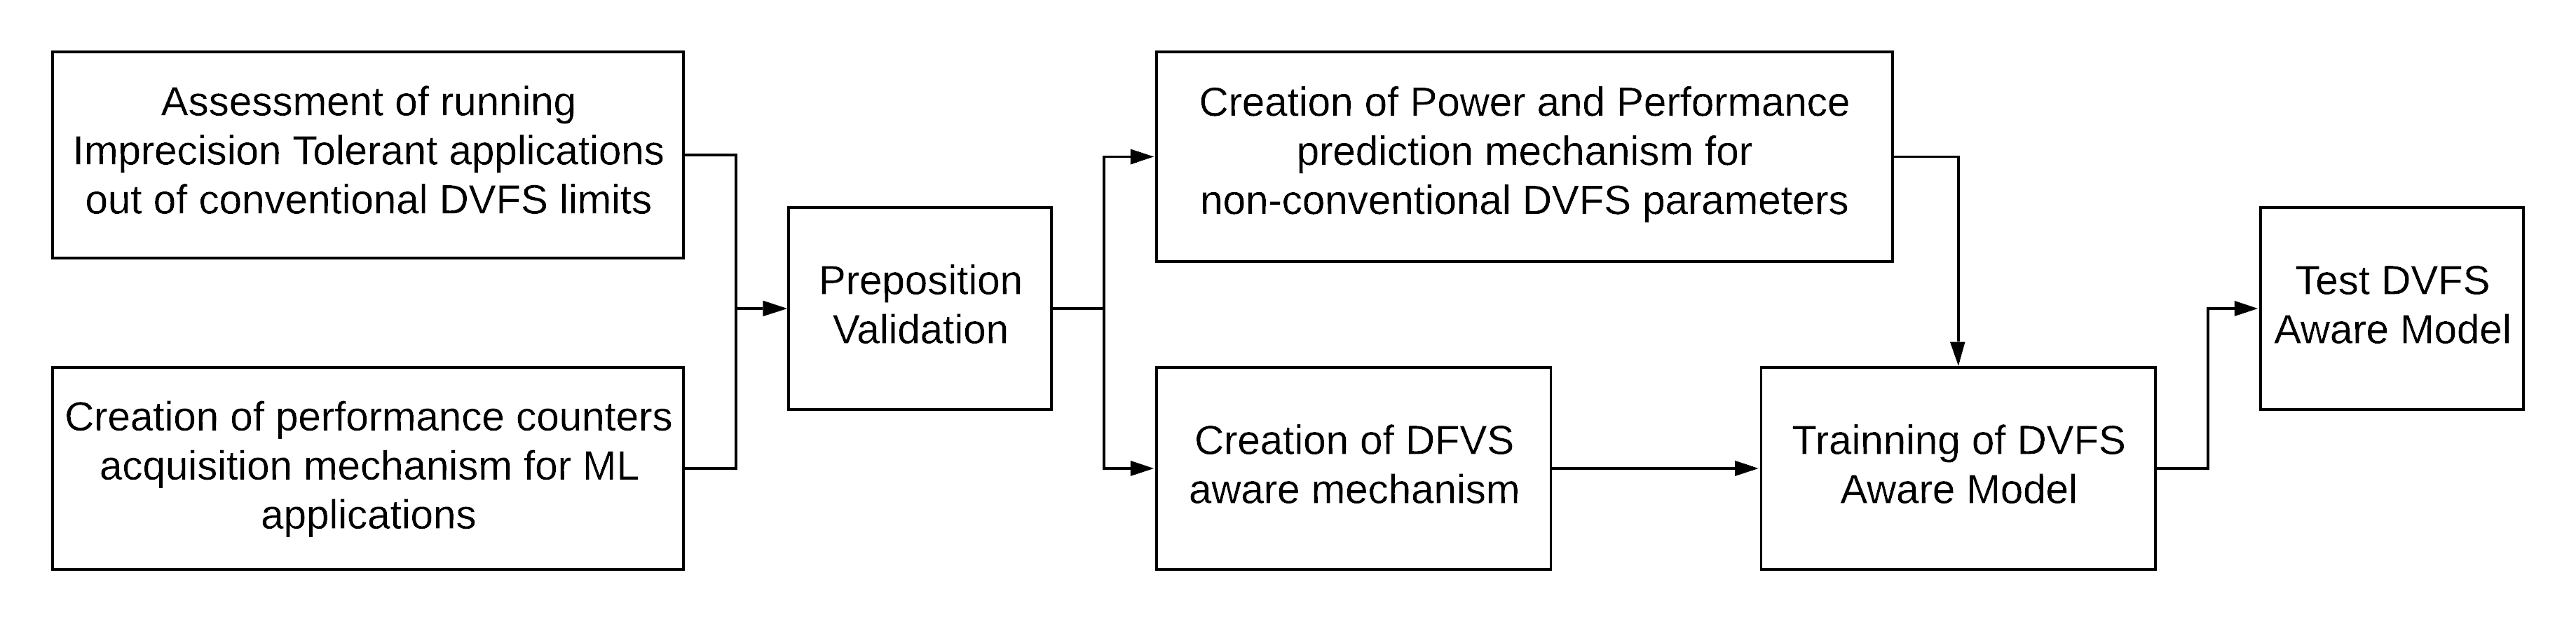
\includegraphics[width=1\textwidth]{Figures/Introduction/Dissertation_Objectives.png}
  \caption{Flowchart of dissertation objectives.}
  \label{fig:thesisObj}
\end{figure}

\section{Report Outline}